\documentclass[psamsfonts]{amsart}

%-------Packages---------
\usepackage{amssymb,amsfonts}
\usepackage{semantic}
\usepackage{fullpage}
\usepackage{tikz-cd}
\usepackage{todonotes}
\usepackage{physics}
\usepackage[all,arc]{xy}
\usepackage{enumerate}
\usepackage{enumitem}
\usepackage{mathrsfs}
\usepackage{theoremref}
\usepackage{graphicx}
\usepackage[bookmarks]{hyperref}

%--------Theorem Environments--------
%theoremstyle{plain} --- default
\newtheorem{thm}{Theorem}[section]
\newtheorem{cor}[thm]{Corollary}
\newtheorem{prop}[thm]{Proposition}
\newtheorem{lem}[thm]{Lemma}
\newtheorem{conj}[thm]{Conjecture}
\newtheorem{quest}[thm]{Question}

\theoremstyle{definition}
\newtheorem{defn}[thm]{Definition}
\newtheorem{defns}[thm]{Definitions}
\newtheorem{con}[thm]{Construction}
\newtheorem{exmp}[thm]{Example}
\newtheorem{exmps}[thm]{Examples}
\newtheorem{notn}[thm]{Notation}
\newtheorem{notns}[thm]{Notations}
\newtheorem{addm}[thm]{Addendum}
\newtheorem{exer}[thm]{Exercise}
\newtheorem{innercustomexer}{Exercise}
\newenvironment{customexer}[1]
  {\renewcommand\theinnercustomexer{#1}\innercustomexer}
  {\endinnercustomexer}

\newtheorem{innercustomprob}{Problem}
\newenvironment{customprob}[1]
  {\renewcommand\theinnercustomprob{#1}\innercustomprob}
  {\endinnercustomprob}

\newtheorem{innercustomthm}{Proposition}
\newenvironment{customthm}[1]
  {\renewcommand\theinnercustomthm{#1}\innercustomthm}
  {\endinnercustomthm}

\theoremstyle{remar}
\newtheorem*{rem}{Remark}
\newtheorem{rems}[thm]{Remarks}
\newtheorem{warn}[thm]{Warning}
\newtheorem{sch}[thm]{Scholium}

\DeclareMathOperator{\Hom}{Hom}
\DeclareMathOperator{\Id}{Id}
\DeclareMathOperator{\End}{End}
\DeclareMathOperator{\ord}{ord}
\DeclareMathOperator{\Aut}{Aut}
\DeclareMathOperator{\Gal}{Gal}
\DeclareMathOperator{\RP}{\mathbb{R}\mathbb{P}}
\DeclareMathOperator{\CP}{\mathbb{C}\mathbb{P}}
\DeclareMathOperator{\Int}{Int}
\DeclareMathOperator{\bd}{bd}
\DeclareMathOperator{\supp}{supp}
\DeclareMathOperator{\sgn}{sgn}

\makeatletter
\let\c@equation\c@thm
\makeatother
\numberwithin{equation}{section}

\bibliographystyle{plain}

\begin{document}

\title{Algebraic Topology II Lecture Notes}
\author{Hidenori Shinohara}

\maketitle
\tableofcontents

\section{Poincare Duality}

Since $H^{\ast}(T^n) \equiv \wedge_{\mathbb{Z}} M$ where $M = \ev{ v_1, \cdots, v_n }$, we have

\begin{center}
  \begin{tabular}{| l | l | l | l | l | l | l |} \hline
    $k$                          & 0 & 1 & 2 & $\cdots$ & $n - 1$  & $n$ \\ \hline
    $\rank H^k(T^n; \mathbb{Z})$ & $\binom{n}{0}$ & $\binom{n}{1}$ & $\binom{n}{2}$ & $\cdots$ & $\binom{n}{n - 1}$ & $\binom{n}{n}$ \\ \hline
  \end{tabular}
\end{center}

This symmetry phenomenon is true in general and very useful.
Another example: The cellular complex for $\CP^n$ is $\mathbb{Z} \rightarrow 0 \rightarrow \mathbb{Z} \rightarrow 0 \rightarrow \cdots \rightarrow 0 \rightarrow \mathbb{Z} \rightarrow 0$.
Thus

\begin{center}
  \begin{tabular}{| l | l | l | l | l | l | l |} \hline
    $k$                          & 0 & 1 & 2 & $\cdots$ & $2n - 1$  & $2n$ \\ \hline
    $\rank H^k(\CP^n; \mathbb{Z})$ & 1 & 0 & 1 & $\cdots$ & 0         & 1 \\
    \hline
  \end{tabular}
\end{center}

\subsection{Orientations}

\begin{defn}
  Let $M$ be a triangulable closed $n$-manifold.
  Let $\sigma_1, \cdots, \sigma_k$ be $n$-simplices such that $M = \sigma_1 \cup \cdots \cup \sigma_k$.
  Then $\sigma_i \in C_n(M)$ for each $i$.
  Suppose that the ordering of the vertices in $\sigma_i$ and the signs $\pm$ can be chosen such that
  \begin{align*}
    \sum \pm \partial \sigma_i = 0 \in C_{n - 1}(M).
  \end{align*}
  Then $M$ is said to be \textit{orientable}.
\end{defn}

\begin{exmp}
  A tetrahedron and torus are examples of orientable manifolds.
  \begin{figure}[!htb]
    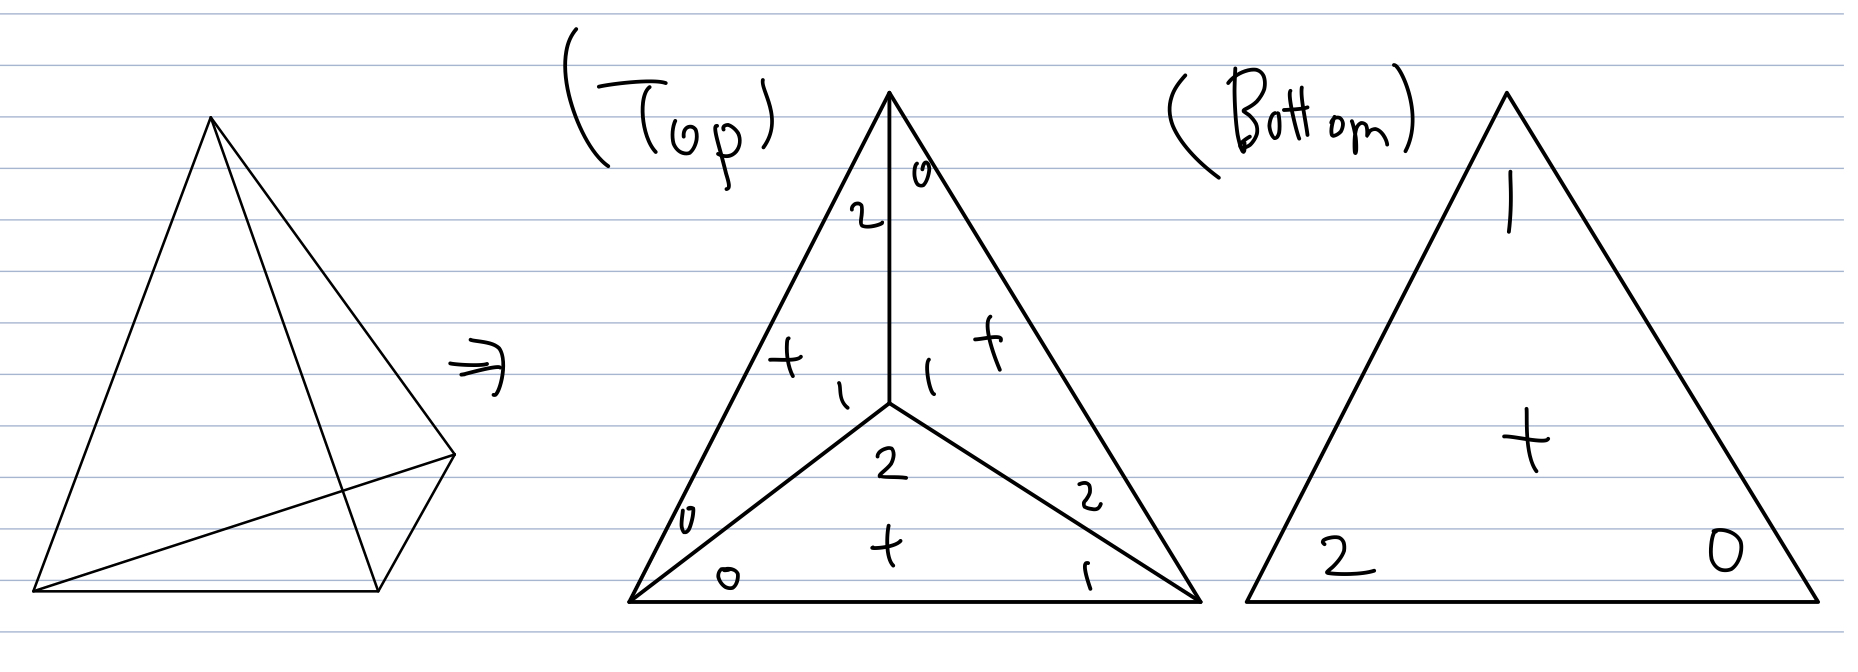
\includegraphics[width=.5\linewidth]{img/orientation_tetrahedron.jpeg}
    \caption{Orientation of a tetrahedron}
    \label{fig:orientation_tetrahedron}
  \end{figure}
\end{exmp}

\begin{defn}
  Let $M$ be an $n$-dimensional orientable manifold.
  Choose $\sigma_i \in C_n(M)$ and signs $\sgn_i \in \{ -1, 1 \}$ such that $M = \sigma_1 \cup \cdots \cup \sigma_k$ and $\sum \sgn_i \partial \sigma_i = 0$.
  The class represented by $\sum \sgn_i \sigma_i \in \ker(\partial)$ in $H_n(M)$ is called a fundamental class $[M]$.
\end{defn}

\begin{thm}\label{fundamental_class_generator}
  If $M$ connected, then $[M]$ is a generator of $H_n(M)$.
\end{thm}

\begin{proof}
  By Poincare Duality(which will be discussed later (\ref{poincare_duality_1})), $H_n(M) \cong H^0(M) = \mathbb{Z}$.
  Let $\sum c_i \sigma_i$ represent a generator of $H_n(M)$ where $c_i \in \mathbb{Z}$.
  Then $\sum \sgn_i \sigma_i = \lambda\sum c_i \sigma_i = \sum (\lambda c_i) \sigma_i$ for some $\lambda \in \mathbb{Z}$.
  Since each $\lambda c_i = \sgn_i \in \{ -1, 1 \}$, $\lambda$ must be 1 or -1.
  Therefore, the class represented by $\sum \sgn_i \sigma_i$ is a generator of $H_n(M)$.
\end{proof}

\begin{cor}
  There are two fundamental classes for any connected orientable manifold.
\end{cor}

\begin{proof}
  By (\ref{fundamental_class_generator}), a fundamental class $[M]$ is a generator of $H_n(M) = \mathbb{Z}$.
  Since $\mathbb{Z}$ has exactly two generators $1, -1$, $M$ has exactly two fundamental classes.
\end{proof}

\begin{defn}
  Let $M$ be a connected, orientable manifold.
  Then a choice of a fundamental class is called an orientation of $M$.
\end{defn}

\subsection{Poincare Duality(Version 1)}

\begin{thm}\label{poincare_duality_1}
  If $M$ is an orientable closed $n$-manifold, then
  \begin{align*}
    H^k(M; G) \cong H_{n - k}(M; G)
  \end{align*}
  for any integer $0 \leq k \leq n$ and an abelian group $G$.
\end{thm}

\begin{rem}
  If $M$ is not orientable, Poincare Duality holds when $G = \mathbb{Z} / 2$.
  In other words,
  \begin{align*}
    H^k(M; \mathbb{Z} / 2) \cong H_{n - k}(M; \mathbb{Z} / 2).
  \end{align*}
  For instance,
  \begin{center}
    \begin{tabular}{| l | l | l | l |} \hline
      $H_{\ast}(\RP^2; \mathbb{Z})$ & 0                & $\mathbb{Z} / 2$ & $\mathbb{Z}$ \\ \hline
      $H^{\ast}(\RP^2; \mathbb{Z})$ & $\mathbb{Z} / 2$ & 0                & $\mathbb{Z}$ \\ \hline
    \end{tabular}
  \end{center}
  so Poincare Duality does not hold in this case.
  However, with $\mathbb{Z} / 2$,
  \begin{center}
    \begin{tabular}{| l | l | l | l |} \hline
      $H_{\ast}(\RP^2; \mathbb{Z} / 2)$ & $\mathbb{Z} / 2$ & $\mathbb{Z} / 2$ & $\mathbb{Z} / 2$ \\ \hline
      $H^{\ast}(\RP^2; \mathbb{Z} / 2)$ & $\mathbb{Z} / 2$ & $\mathbb{Z} / 2$ & $\mathbb{Z} / 2$ \\ \hline
    \end{tabular}
  \end{center}
  so Poincare Duality holds in this case.
\end{rem}

\begin{defn}
  The $k$th Betti number of a manifold $M$ is defined to be $b_k = \rank(H^k(M; \mathbb{Z}))$.
\end{defn}

\begin{thm}
  $b_k = b_{n - k}$ for all $k$ if $M$ is a closed orientable $n$-manifold.
\end{thm}

\begin{proof}
  By the Universal Coefficient Theorem, $\rank(H^k(M)) = \rank(H_k(M))$.
  By Poincare Duality, $\rank(H^k(M)) = \rank(H_{n - k}(M))$.
  Therefore, $b_k = \rank(H^k(M)) = \rank(H_{n - k}(M)) = \rank(H^{n - k}(M)) = b_{n - k}$.
\end{proof}

\subsection{Cap Products}
There is a nice way to explicitly write down the isomorphism when $G$ is a commutative ring.

\begin{defn}
  Let a space $X$ and a commutative ring $R$ be given.
  For any $k \geq l$, define the cap product
  \begin{center}
    \begin{tikzcd}[cells={nodes={minimum height=2em}}]
      \frown: & C_k(X; R) \otimes C^l(X; R) \arrow[r] & C_{k - l}(X; R) \\
              & \sigma \otimes \phi \arrow[r, maps to]         & \phi(\sigma\vert_{[v_0,\cdots,v_l]})\sigma\vert_{[v_l, \cdots, v_k]}
    \end{tikzcd}
  \end{center}
\end{defn}


\end{document}
